%------------------------------------%
% Début Partie Azarias				%
%------------------------------------%
\part{System design}
\chapter{User interface design}
Because the project was created with Qt, and Qt it adapts its interface depending on the OS it is running on, there is no \textit{global} user interface. However, the layout is always the same and so is the content. The following screenshots will show the user interface as it is on Linux, more precisely Ubuntu. Currently, QTypingTest is available on Ubuntu, Windows and Mac OS.\\
When the user starts the software, they are directed to the homepage, (figure \ref{homepage-logout}) where they can either create a new profile or connect to their own existing profile. The buttons to go through the different parts of the software are disabled as long as no one is connected. A list of the existing users is displayed and the user just has to click on their alias to connect (figure \ref{homepage-login}). They can then go through the different parts of the user interface. 
\begin{figure}[H]
  \centering
  \begin{minipage}[b]{0.45\textwidth}
    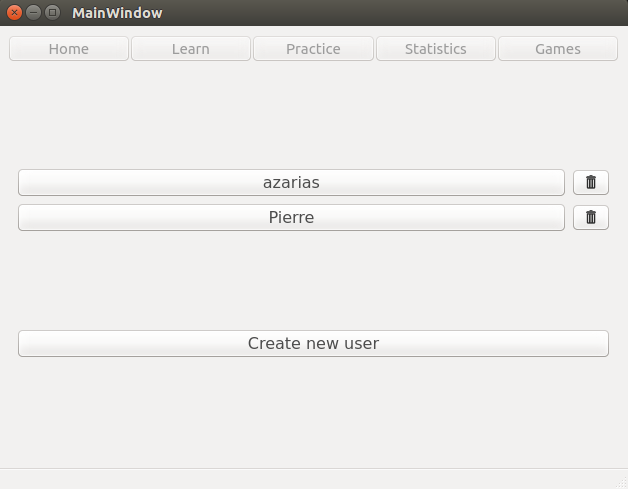
\includegraphics[width=\textwidth]{images/homepage_logout.png}
    \caption{The default homepage.}
    \label{homepage-logout}
  \end{minipage}
  \hfill
  \begin{minipage}[b]{0.45\textwidth}
    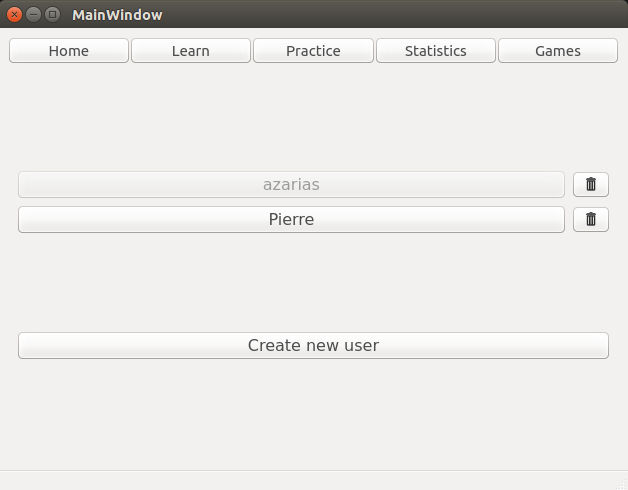
\includegraphics[width=\textwidth]{images/homepage_login.png}
    \caption{When the user is connected.}
    \label{homepage-login}
  \end{minipage}
\end{figure}
A user can also delete their profile by clicking on the trash icon. \\
The login system does not need to be secured. Since this software is intended for private use, and because it does not contain any sensitive information, the group decided to focus on the software itself and to do not spend too much time on the login system. \\
On the top of the window, there are five buttons.
\begin{itemize}
	\item Home. This button, when triggered, shows the homepage, but does not disconnect the user.
	\item Learn. This shows the main part of the project. The page where the user sees a list of the different letters to learn in an certain order.
	\item Practice. On this page, the user can choose different modes of practice.
	\item Statistics. Here, the user can see their statistics.
	\item Games. A simple game developed to learn fun ways to type.
\end{itemize}


\begin{figure}[H]
	\centering
	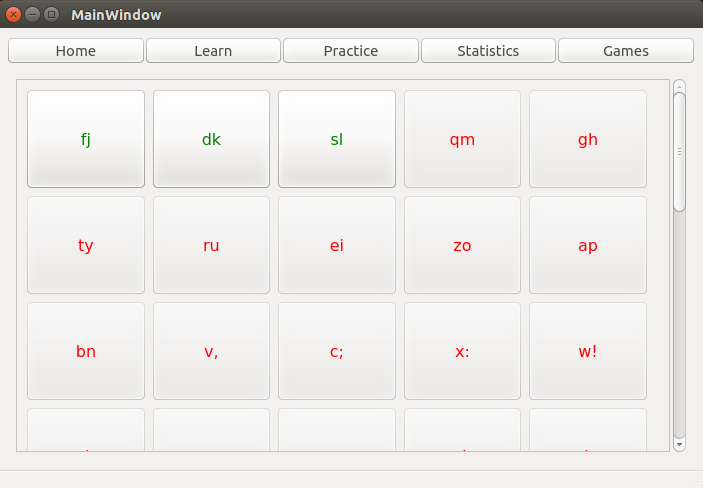
\includegraphics[width=0.7\textwidth]{images/page-learn.png}
	\caption{Learn page}
	\label{page-learn}
\end{figure}

In the learn page (figure \ref{page-learn}) the user can see all the exercises to come. They must succeed through each stage one by one and reach a minimum score the be able to unlock the next exercise. When clicking on a button, a dialog is shown and the user can start a new exercise.

\begin{figure}[H]
	\centering
	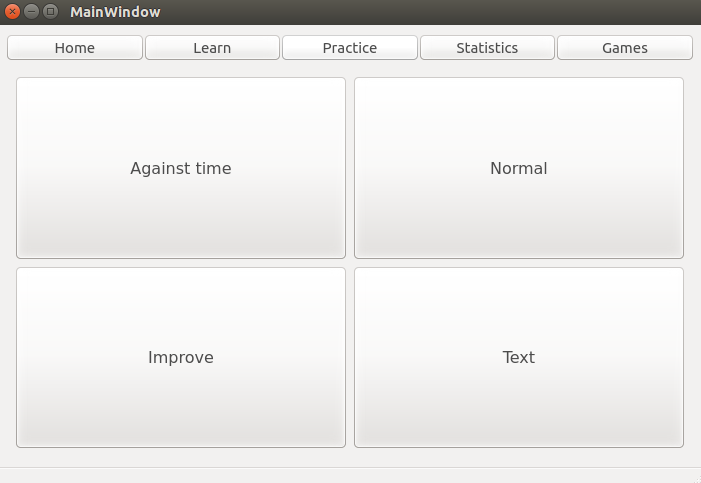
\includegraphics[width=0.7\textwidth]{images/page-practice.png}
	 \caption{Practice page}
	 \label{page-practice}
\end{figure}

The practice page  (figure \ref{page-practice}) has four buttons, one for each different type of practice exercises. The overall appearance of each practice exercise is always the same : a dialog with a text to type. What changes is the content of the dialog.\\
The different rules for each type of practice are 
\begin{description}[align=left]
	\item[Against time/Race :] The user must type the most words in one minute. At the end of the minute, the number of words per minute is shown.
	\item[Normal :] The user has two slides of random words to type. Thanks to the powerful language system of Qt, the displayed words may vary depending on the user's computer language. For the moment, only english and french are supported.
	\item[Improve :] This practice will check what are the user's worst letters and create a special exercise containing these letters.
	\item[Text :] In this practice, the user will have to type an existing text. The chosen text is from classical authors such as George Orwell. Once again thanks to Qt, the language of the text may vary depending on the user's computer language. The default language being english. Currently the languages available are english and french.
\end{description}

%\textit{The statistics page was not made yet}

\begin{figure}[H]
	\centering
	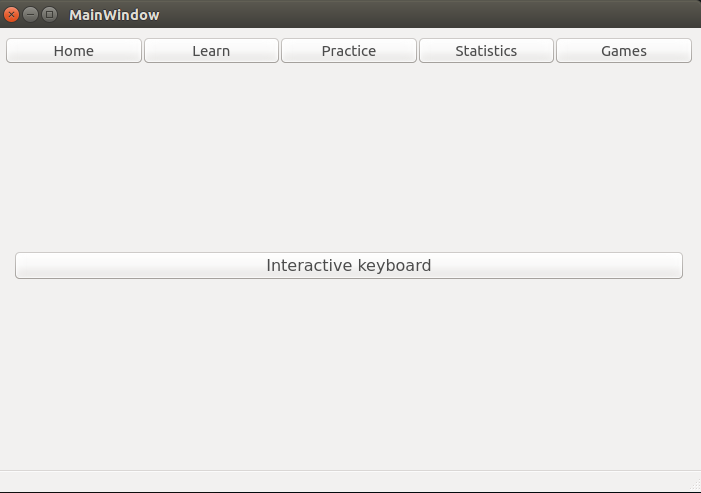
\includegraphics[width=0.7\textwidth]{images/page-games.png}
	 \caption{Game page}
	 \label{page-game}
\end{figure}

The game page (figure \ref{page-game}) contains a single button. This button launches a dialog where the user sees what letters are associated with what finger on the keyboard. They just have to type a letter on the keyboard and the letter on the virtual keyboard will highlight as well as its associated finger on the bottom of the dialog.

\subsection{The differents dialogs}
Here are the dialogs that can be opened in QTypingTest :

\begin{figure}[H]
	\centering
	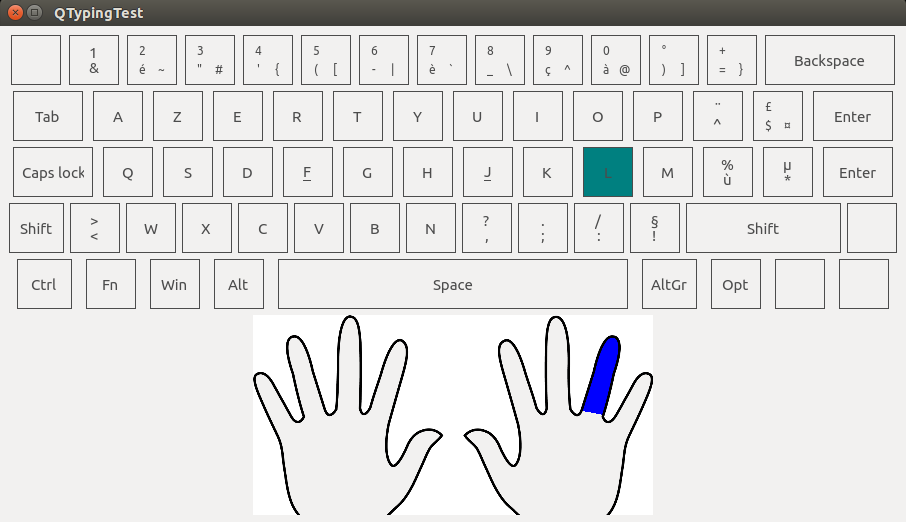
\includegraphics[width=0.7\textwidth]{images/dialog-before-learn.png}
	 \caption{Before the learning dialog}
	 \label{dialog-before-learn}
\end{figure}

Here is the dialog shown when the user starts an exercise to learn new letters.\\
This dialog highlights in a certain color the finger along with the letter on the keyboard. This invites the user to do the same and thus using the indicated finger to type on the indicated letter. When they do this, the next letter and the next finger highlights. When those two steps are completed, the user can start the real exercise.\\
The pictures show the configuration of an AZERTY keyboard, because the test are made on a french computer. But a configuration file is also made for QWERTY keyboard, and anyone who uses a non-french computer's configuration will automatically have the QWERTY configuration loaded. Since this is the default configuration (and the most used worldwide).

\begin{figure}[H]
	\centering
	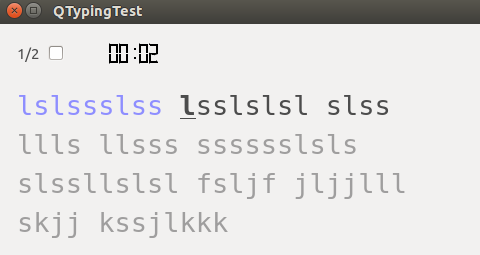
\includegraphics[width=0.7\textwidth]{images/dialog-learn.png}
	 \caption{The learning dialog}
	 \label{dialog-learn}
\end{figure}

The figure \ref{dialog-learn} shows the dialog to learn new letters. In this case, the letters are \textit{S} and \textit{L}.\\
There are two parts in the dialog : the toolbar and the center part.\\
The toolbar contains :
\begin{itemize}
	\item The page indicators tells what page the user is located and how many pages remain.
	\item The play/pause button is the checkbox button. When it is toggled the game is paused and when it is not (the default) the game goes on.
	\item The timer. This tells the user how much time was spent since the start of the exercise or how much time remains before the end of the exercise when practising against time.
\end{itemize}

The center part contains the user's exercise. It displays a text on two pages with four color codes :
\begin{itemize}
	\item Black : a normal black letter is a letter to be typed in the future
	\item Black underlined and bold : the current letter that the user has to type
	\item Blue : a letter already typed by the user and correctly typed
	\item Red  : a letter already typed by the user but incorrectly typed
\end{itemize}

The center part does not take care of the words. It only takes care of each letter.\\
The user can rewind back to retype the letters. This will also work from one line to another. However this is voluntary it is not possible from one slide to another.\\
This dialog will always look the same for the trainings and the exercise. The only difference lives in the content of the main part.\\
For the exercise dialog, the exercise is organized as so :
\begin{enumerate}
	\item For two lines, only the two letters that the user must learn.
	\item For two lines all the letters previously learned in a random order
	\item And the remaining part one some random words with the letters previously learned. If no words can be made with the letters learned (especially true at the beginning) the second part will be repeated.
\end{enumerate}

\begin{figure}[H]
	\centering
	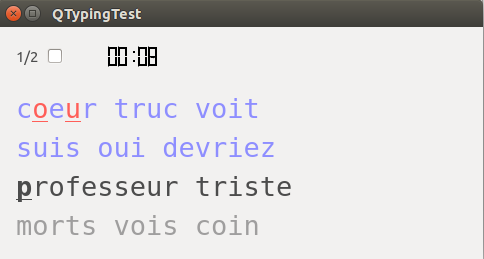
\includegraphics[width=0.7\textwidth]{images/dialog-practice.png}
	 \caption{The practice dialog}
	 \label{dialog-practice}
\end{figure}

This dialog is very similar to the learning dialog. The toolbar is exactly the same and works the same way.\\
The only difference is the content. This dialog contains only real words. In this case, it is only french words since there is a file containing french words for french computers. There is also a file containing english words. And this file is the default one.\\
This type of exercise contains only words placed in a random order, on two slides.

\begin{figure}[H]
	\centering
	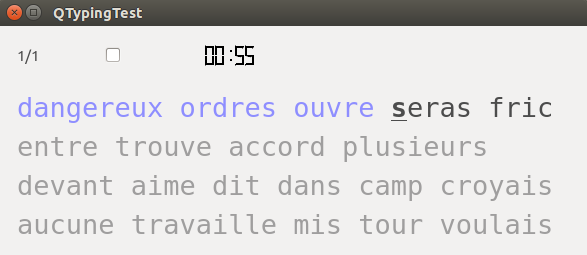
\includegraphics[width=0.7\textwidth]{images/dialog-race.png}
	 \caption{The race dialog}
	 \label{dialog-race}
\end{figure}

The race dialog is similar to the two previous ones. However there is one difference in the toolbar. Instead of starting at 0, the timer starts at 1 minute, and decreases. This will result in another change i.e the number of pages. The number of pages depends on the speed of the user. It is 'unknown'. However, instead of hiding this information, it will simply increase for each new page created.\\
For this exercise, only one page is generated and if the user completes the page, another one is generated and displayed. Thanks to the speed of C++ and the algorithms developed by the group, the user does not see the difference. This system allows the exercise to generate (in theory) an infinite number of pages and therefore change the start time.
The content is the same as the practice dialog : it contains only words in french or english depending on the user's computer (in this case, french).\\

\begin{figure}[H]
	\centering
	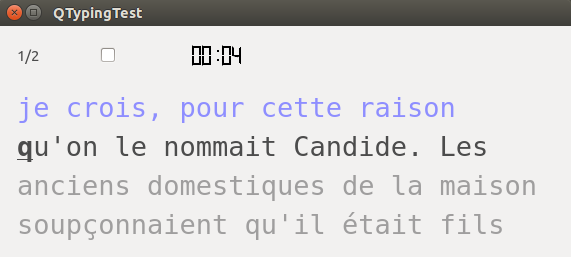
\includegraphics[width=0.7\textwidth]{images/dialog-text.png}
	 \caption{The text dialog}
	 \label{dialog-text}
\end{figure}

The text dialog is exactly the same as the practice dialog. The only difference is the content. Instead of containing only random words, it contains real text. The text is either in french or english, depending on the user's computer configuration. The default language for the text is english.

\begin{figure}[H]
	\centering
	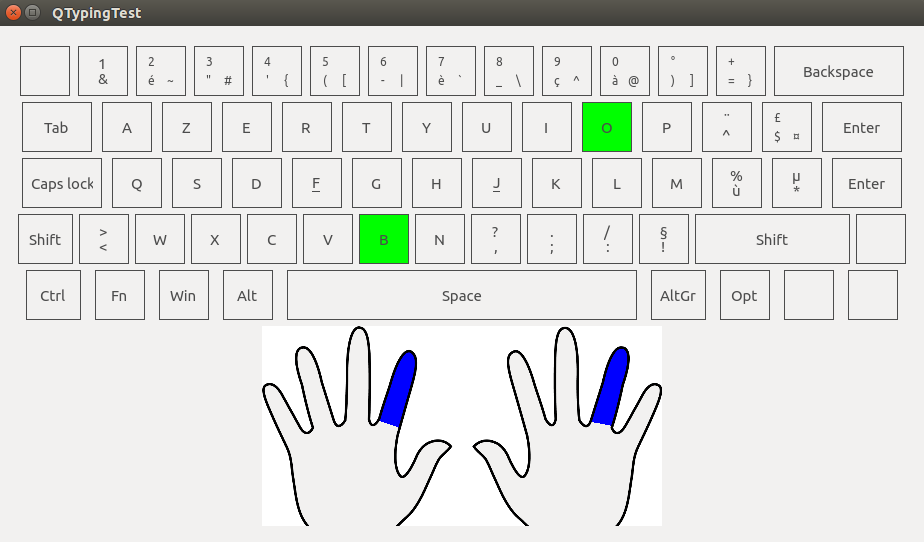
\includegraphics[width=0.7\textwidth]{images/dialog-game.png}
	 \caption{The game dialog}
	 \label{dialog-game}
\end{figure}

The game dialog is the same as the one shown before the learning exercise. However instead of showing the user what letter they have to type, it will simply allow them to type whatever letters they want, and show what finger is associated with this letter. \\

\section{Qt features}

Qt is a really powerful framework packed full of features. There are so many of them that it is sometimes possible to miss one and recreate something pre-existing within Qt. That is what happened for the group many times during the development of the software.\\
Qt is first made to create user interfaces on a variety of OS. With the same source code, it is possible to have a interface for linux, windows and mac OS. But there are lots of useful features to improve the life of the developer and some tools to improve the C++ language.\\
The most powerful feature by far of Qt is it's SIGNAL-SLOT system.

\begin{figure}[H]
	\centering
	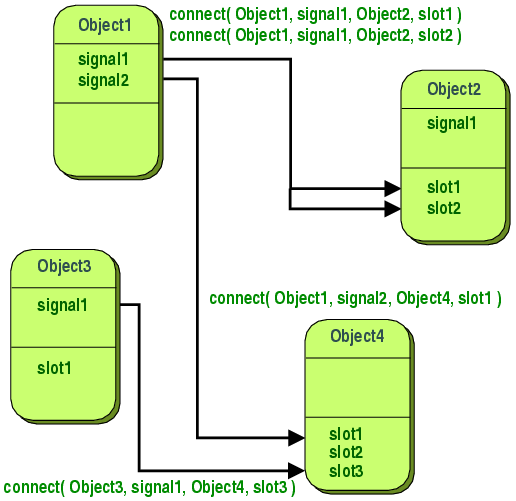
\includegraphics[width=0.7\textwidth]{images/abstract-connections.png}
	 \caption{The connection system in Qt}
	 \label{signal-slot-qt}
\end{figure}

The figure \ref{signal-slot-qt} shows how it works. A signal can be emitted and a slot can be called whenever a signal is emitted. This is very useful to program interactive user interfaces.\\
It would be too long to enumerate all the features that Qt provides, and a lots of them were not used in the project. However, here is a list of features used for the project provided by Qt.

\begin{description}[align=left]
	\item[Language detection] : Qt can easily detect the user's computer language. This was first used to select the files for the exercises. It is possible to get the language of the computer as a string and then choose what file to parse depending on this string.
	\item[Resources files] : The group discovered later than Qt can actually automatically select the good file depending on the computer language. This is thanks to a resource file (.qrc). This file is written in XML and tells Qt where to find the resource file, given them a language and an alias. Then, when needing a file in the code the alias of the file is given, and Qt will choose the good file depending on the computer's language.
	\item[DataStream] : It is possible with Qt to open and read or write in a file. This was first used to save the users in binary files. The files can also be opened in text mode to read and write UTF8-only characters. This was first used to read the keyboard configuration files.
	\item[QSettings] : As for the language detection, the group discovered later that Qt has a pre-made data-saving system. This provides a safer way to save the data on the computer. Instead of writing on a file in the folder of the project itself, Qt will choose a system folder depending on the OS of the computer to write down the data to save.
	\item[Json] : Qt supports the JSON format. It can parse any valid JSON file and be used later on in the code. This is what is actually used to save the keyboard configurations. 
	\item[XML] : As for the JSON, Qt also supports XML. It can parse any XML file and return an object that can be manipulated easily. This features can be used to save the texts.
	\item[QString] : Last be not least. Qt provides a really powerful class : the QString. This class is really easy to use, and full of functions. It is like the String class in Java : a string of characters.
\end{description}

\subsection{Documentation}
It is not a part of Qt itself, but without it, the development of the software would be impossible.\\
The documentation of Qt is available online, but also on QtCreator. It is really well-made, easy to read, comprehensive, completed with examples and consistent. The documentation is always up-to-date and any depreciated feature is always replaced with something more convenient to use.\\
Moreover, when there is a problem with Qt and the documentation cannot solve the problem, the community behind Qt is huge and really helpful. Qt itself has a special forum to ask questions about the framework. There is also famous forum StackOverflow. Those two forums helped the group many times when having a problem with Qt.

\chapter{Functional Design}
This project is relatively simple and contains two main parts :
\begin{description}
	\item[The learning] : where the user learn each letter of the keyboard one by one
	\item[The practising] : where the user can see the progress made by typing real words, and real texts
\end{description}
Since this software is quite simple, everyone with a computer can use it. This means the software is made for all ages. Anyone no matter how old they are, can use the software without a lot of explanations and learn, step by step how to correctly use his keyboard.\\
Also, thanks to Qt robustness and features, the software is viable and is unlikely to crash during use.

\section{Structure of the system}

\begin{itemize}
	\item The Data part. This part contains classes where data are stored. e.g the users, his statistics... Data part contains also the user manager, used to manage user's connection and disconnection.
	\item The User interface part. This part contains all the files necessary to create the user interface. All classes in this parts inherits at least of QWidget (which is the base element for the GUI).
	\item The utils part. This part only contains namespaces. These class facilitates developer's life and provides useful functions to make the software work.  
\end{itemize}

Those three parts are separated in three different folders (namely "Data","QTypingpTest" and "Utils").\\
This separation was creating a pseudo-pattern of MVC. The model being the data, the View being the GUI and the Utils being the controller. However, for programming reasons, the main parts of the controller are in the view itself. Thanks to the signal slot (figure \ref{signal-slot-qt}) system, the function used as controller is in the GUI itself.

\section{Style of code}
To have an homogeneous code, the group decided to follow some rules for the style of code. The choose the google C++ style guide. The website for this style guide is the following : \url{https://google.github.io/styleguide/cppguide.html}.
The document is quite long and some rules are more obvious than others. Here is a reduced list of the notable rules that the group followed :
\begin{itemize}
	\item \href{https://google.github.io/styleguide/cppguide.html#Access_Control}{Access-control}. Make data member of a class private. 
	\item \href{https://google.github.io/styleguide/cppguide.html#Write_Short_Functions}{Write short functions} No more than 40 lines if possible.
	\item \href{https://google.github.io/styleguide/cppguide.html#Use_of_const}{Use const} whenever it makes sense.
	\item \href{https://google.github.io/styleguide/cppguide.html#auto}{Use auto keyword}. C++11 introduced the auto keyword, allowing to reduce the long and cumbersome type names.
	\item \href{https://google.github.io/styleguide/cppguide.html#Variable_Names}{Variable names}. Name of variable are lower case. With a trailing underscore at the end of the private data members.
	\item \href{https://google.github.io/styleguide/cppguide.html#File_Names}{File names}. Name the file in lower case.
\end{itemize}
All these rules were not followed entirely. Indeed the rules enumerated above apply to the C++ in general and in this case, the group used Qt which is a different environment from usual C++ one. A simple example is for the variable name. C++ style guide advises to use a name with only lower-case letters, joined with underscore. But the Qt style guide prefers to call the variable camel-cased.

\section{Code walkthrough}


\subsection{The main file}
Begin with the beginning : the main.
\begin{lstlisting}
#include <QApplication>//The application
#include <QDebug>//The logger
#include <QDir>
#include <time.h>//Random number 
#include <QFile>
#include <QTranslator>//Computer's locale
#include <QLocale>
#include <QLibraryInfo>

#include "QTypingTest/thomepage.h"

void init(){
    srand(time(NULL)); //Random number generation

    qRegisterMetaTypeStreamOperators<TUser>("TUser"); //Metatype declaration

    //Set translator
    QString locale = QLocale::system().name().section('_',0,0);
    QTranslator translator;
    translator.load(QString("qt_") + locale,QLibraryInfo::location(QLibraryInfo::TranslationsPath));
    QApplication::installTranslator(&translator);
}


int main(int argc, char *argv[]) {
    QApplication a(argc, argv);//Start Qt

    init();   //Register the type to be able to create QVariant from them

    THomePage hp;

    //Set style
    QFile file(":/style.qss");
    if (file.exists()) {
        if (!file.open(QIODevice::ReadOnly | QIODevice::Text)) {
            qDebug() << "Could not open file, please check the permissions";
        } else {
            hp.setStyleSheet(QLatin1String(file.readAll()));
        }
        file.close();
    } else {
        qDebug() << "Could not load stylesheet";
    }


	//Show the main window
    hp.show();

	//enter qt's main loop
    return a.exec();
}
\end{lstlisting}

This code is very interesting since it shows a lot in a few lines of code. Here is step by step, what is happening :
\begin{description}
	\item[Creating the qt application object.] To run qt, an application must be created, otherwise, there is no main loop and no window to display
	\item[init().]  This function contains a series of initialisation :
	\begin{itemize}
		\item Initiate the random number generation
		\item Register the TUser type to be able to read saves
		\item Detect the computer language
		\item Install the translator of the detected language.
	\end{itemize}
	\item[Set the style.] Qt support the CSS format. This style can be applied to the elements of the GUI. Since almost all basics CSS directives are supported, it was easy to customize the GUI.
	\item[Show the main window.] The homepage was already created before. As all initialisations are done, it is possible now to display it.
	\item[Enter the main loop.] To let the window open and really launch the software once for all. The last line does this for us.
\end{description}


\subsection{A widget class}
\begin{lstlisting}
void THomePage::connectEvents() {
    TUserManager::getInstance().readUsers();
    connect(ui.action_option,SIGNAL(triggered(bool)),this,SLOT(showOptionDialog()));
    connect(ui.action_aboutQt,SIGNAL(triggered(bool)),qApp,SLOT(aboutQt()));
    connect(&TUserManager::getInstance(),&TUserManager::usersSaved,this,[=](){
        ui.statusbar->showMessage("Users saved !",4000);
    });
    connect(&TUserManager::getInstance(),SIGNAL(userChanged(TUser*)),this,SLOT(updateUI(TUser*)) );

	//Associate 
    buttonsStacks_[ui.button_home] = ui.page_home;
    buttonsStacks_[ui.button_learn] = ui.page_learn;
    buttonsStacks_[ui.button_games] = ui.page_games;
    buttonsStacks_[ui.button_stats] = ui.page_stats;
    buttonsStacks_[ui.button_practice] = ui.page_practice;

    //Iterate over the buttons-page couple
    for (auto it = buttonsStacks_.begin(); it != buttonsStacks_.end(); ++it) {
        //If child is not nullptr create a simple layout with parent and add the child into it
        if (!TUserManager::getInstance().getCurrentUser()) {
            it.key()->setEnabled(false);
        }

        connect(it.key(), &QPushButton::clicked, [ = ](){
            ui.stack_main->setCurrentWidget(it.value());
        });
    }
    ui.stack_main->setCurrentWidget(ui.page_home);
}
\end{lstlisting}
This function is called in the constructor of the main window. The interesting thing here is the signal-slot system of Qt.
Here is the list of what this function does :
\begin{description}
	\item[Read the users.] Loads the QSettings saved from the previous session into the usermanager
	\item[Connect the toolbar actions.] The toolbar contains actions connected to several function of the main window
	\item[Associate the buttons with the pages.] The main window contains differents buttons. Each one is changing the current page.
	\item[Show the homepage.]
\end{description}

The signal-slot is used in this function. This line : 
\begin{lstlisting}
connect(&TUserManager::getInstance(),SIGNAL(userChanged(TUser*)),this,SLOT(updateUI(TUser*)) );
\end{lstlisting}
is a connection example. It means : on the instance of Usermanager, when the signal 'userChanged' is emitted, Qt will trigger the function 'updateUI' of the main window.\\
There are several ways to connect a signal to a slot. Another way is shown in the above code with the anonymous function. C++11 introduced the anonymous functions. It is possible to use it as so in Qt :
\begin{lstlisting}
connect(it.key(), &QPushButton::clicked, [ = ](){// < start of anonymous function
	ui.stack_main->setCurrentWidget(it.value());
});//< end of anonymous function
\end{lstlisting}

Many of the widget looks like this : connect the events to custom functions at the initialization , then process the data in those functions.

\subsection{A data class}

The data classes are a bit different from the widget class. The code bellow is the content of the file tuser.h. The header file for the TUser class.
\begin{lstlisting}
#ifndef TUSER_H
#define TUSER_H

//includes [...]

struct date_exercice_ {
    QDateTime dateResult;
    TExercice exercice;
};

class TUser : public QObject {

    Q_OBJECT
    
\end{lstlisting}
First, the class must inherit from QObject to be able to emit signals and have slots. There is also the Q\_OBJECT macro to add some attributes to the class.

\begin{lstlisting}
public:
    TUser(QString pseudo = "", QObject *parent = 0) :
        QObject(parent),
        pseudo_(pseudo),
        progress_(new TProgression()),
        statistics_(TStats()){
    }


   //Getters, setters...

    void setSettings(const TUser &user){
        pseudo_ = user.getPseudo();
        layout_ = user.getLayout();
        emit settingsChanged(this);//< emit a signal with the user in parameter
    }
\end{lstlisting}
This part shows one constructor of the class. Getters and setters are also present in this class but most of them are not interesting. However, the setter for the Settings is different. It emits a signal when the settings changed. This allows the developer to connect a slot to this signal to be warned whenever the current user's settings changed. (And update the GUI in consequence).


\begin{lstlisting}
signals:// 'signals' is used as a keywords like 'public' or 'private'
	//Emitted when the statistics of the user changed
    void statsChanged(TUser *);

	//Emitted when the settings of the user changed
    void settingsChanged(TUser *);
\end{lstlisting}
This part shows how the signal are declared. There is nothing more than this in the .h file. To declare a signal, the only thing to do is declare the function and inform Qt of what argument will be emitted with this function.

\begin{lstlisting}
private:
    QString pseudo_;
    TProgression *progress_;
    TStats statistics_;
    QString layout_;
	QHash<date_exercice_, TResult> practiceHistory_;
\end{lstlisting}
These are the attributes of the TUser class.

\begin{lstlisting}
    friend QDataStream &operator<<(QDataStream& out, const TUser& user){
        out << user.pseudo_ << *user.progress_ << user.statistics_ << user.practiceHistory_ << user.layout_;
        return out;
    }

    friend QDataStream &operator>>(QDataStream& in, TUser &user){
        in >> user.pseudo_ >> *user.progress_ >> user.statistics_ >> user.practiceHistory_ >> user.layout_;
        return in;
    }
};

Q_DECLARE_METATYPE(TUser)
/**
 * Write a user in the DataStream
 * 
 * @param out the dataStream target (where to write the data)
 * @param user the user that is to be written in the dataStream
 * @return the modified dataStream
 */
QDataStream &operator<<(QDataStream& out, const TUser& user);


/**
 * Takes back all the user's informations
 * from the DataStream
 * 
 * @param in the dataStream containing the user
 * @param user the user to initialize from the datastream
 * @return the datastream
 */
QDataStream &operator>>(QDataStream& in, TUser &user);

#endif /* TUSER_H */

\end{lstlisting}
Last but not least, this part of shows how the TUser class is saved in a file. Operators are declared outside of the class and defined in the class with the keyword \texttt{friend} to have access to the private attributes of the TUser passed in argument.

\subsection{A 'util' class}

\begin{lstlisting}
#ifndef FACTORY_H
#define FACTORY_H

//includes[...]

namespace factory {
    
    /**
     * 
     * 
     * This function will read the texts files of the project
     * corresponding to the language.
     * And will keep a random part of the text by keeping 
     * only the asked number of words
     * 
     * @param numbersOfWords the number of words for the text
     * @return a part of a text containing n words, choosen from the file corresponding
     * to the given language. If the file does not exists, english is chosen by default
     */
    QString generateText(int numbersOfWords);

    //[other functions...]

    /**
     * Open and read all the content of a file
     * returns an empty string if the file could not be
     * open
     *
     * @param fileName
     * @return the content of the file (empty if nothing found)
     */
    QString readFile(QString fileName);

}



#endif /* FACTORY_H */
\end{lstlisting}
This is an extract of the factory namespace header. It contains the namespace, and within it, all the functions declaration. The bodies of the functions are in the .cpp file.\\
The aim of these functions is to facilitate developer's life by providing flexible functions which can be used everywhere in the code. These functions only depends of each others, and does not depend of the software itself. (However, the software depends of this functions).\\
All functions of this namespace are fully tested. Tests for these functions was easy because no GUI was required, only functions with inputs and outputs. 

\section{The improved label}
Here is an example of how the label of all the exercise are working. (figure \ref{improved-label} )
\begin{figure}[H]
	\centering
	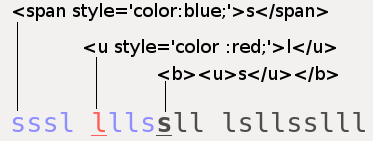
\includegraphics[width=0.7\textwidth]{images/dialog-learn-1.png}
	 \caption{The improved label}
	 \label{improved-label}
\end{figure}
The labels of the exercises dialog uses those differents HTML tags:

\begin{description}
	\item[span] : a simple HTML tag to surround a single character and add style to it
	\item[u] : a HTML tag to underline all its content
	\item[b] : a HTML tag to bold all its content
\end{description}

In addition with these tags, the HTML tag \textit{style} is used. Characters surrounded by this tag are changing depending of it. This is used to set the font color to blue or red.\\
Here is the code of the label when the user typed a letter :
\begin{lstlisting}
bool TLabel::nextChar(bool currendIsCorrect) {
	//Remove all the tags on the current char
    html::removeTag(splitedChars_[currentChar_]);
    if (!currendIsCorrect) {//If not correct, underline and set color to red
        html::addTags(splitedChars_[currentChar_], "u", "style='color : #FF5E58;'");
    } else {//If correct, just set the color to blue
        html::addTags(splitedChars_[currentChar_], "span", "style='color : #8E8EFF';");
    }

	//Go to the next char
    currentChar_++;
    //If some chars remain on the label
    if (currentChar_ < stringToCopy_.size()) {
    		//Underline and bold the current char
        html::addTags(splitedChars_[currentChar_], "b,u");
    }
    this->setText(splitedChars_.join(""));

	//return wether we're at the end of the label
    return currentChar_ < stringToCopy_.size();
}
\end{lstlisting}
This solution is very helpful and allowed the group to easily customize the interface.\\
Then to rewind, the inverted process is used :
\begin{lstlisting}
bool TLabel::previousChar() {
	//If at start, nothing to rewing
    if (currentChar_ == 0)return false;

    if (currentChar_ < splitedChars_.size())
    		//Remove all the tags of the current chars
        html::removeTag(splitedChars_[currentChar_]);

	//Rewing the current char
    currentChar_--;
    //Remove the tags of the current char
    html::removeTag(splitedChars_[currentChar_]);
    //Underline and bold the current char
    html::addTags(splitedChars_[currentChar_], "b,u");
    this->setText(splitedChars_.join(""));
    return true;
}

\end{lstlisting}
Those two functions are relatively simple to understand and therefore easy to maintain. Behind the hood, on the HTML helper, the functions are way more complicated.
Here is the function that surround a char with tags :
\begin{lstlisting}
QString html::addTags(QString &strToTag, QString tags, QString attributes) {
    QStringList splited = tags.split(",", QString::SkipEmptyParts);

    QString res = surroundOfTags(splited, attributes);
    int position = getAbsoluteCharPosition(strToTag, 0);

    QString regex;

    if (position == 0)//If position is at the start
        regex = "(^.)";
    else if (position == strToTag.length() - 1)//If position is the last char
        regex = "(.$)";
    else
        regex = QString("(.)(?=.{%1}$)").arg(strToTag.size() - 1 - position);

    strToTag = strToTag.replace(QRegExp(regex), res);
    return strToTag;
}
\end{lstlisting}

This function is using regular expressions to replace the tag at a certain position. Since this function is much more complicated and crucial for the exercise, it is the first which has been tested.\\

\section{The interactive keyboard}
Another interesting part to see in the code is how the interactive keyboard was implemented.\\
The interactive keyboard contains two main parts :
\begin{itemize}
	\item The upper part, containing the keyboard itself with all the keys in it.
	\item The lower part, containing a drawing of hands.
\end{itemize}
When the user type a letter on his keyboard, a finger will be highlighted as well as a key on the keyboard.\\
The interactive keyboard can also support several keys pressed at once. The only limit is the keyboard itself. Therefore, a mechanic keyboard will be able to visualize more key pressed than a classical keyboard.\\
Four classes are necessary to have the full interactive keyboard working :
\begin{description}
	\item[TFingerPosition : ] this class is the widget that will display the hands on the lower part of the interactive keyboard.
	\item[TVirtualKey : ] this class represent a single key that can be activated.
	\item[TVirtualKeyBoard :] this class is a widget that contains several virtual key representing all the keys the user can interact with.
	\item[TPresentation : ] this class put together the finger position widget and the virtual keyboard widget. So every time a key is pressed, this class will know what finger to highlight.
\end{description}

\begin{lstlisting}
#ifndef TFINGERPOSITION_H
#define TFINGERPOSITION_H

//#include ...


class TFingerPosition : public QWidget {
    Q_OBJECT
public:
    TFingerPosition(QWidget *parent = 0);

    virtual ~TFingerPosition() {
    }

    enum FINGER {
        LEFT_PINKY, LEFT_RING, LEFT_MIDDLE, LEFT_INDEX, 
        RIGHT_INDEX, RIGHT_MIDDLE, RIGHT_RING, RIGHT_PINKY,
        NO_FINGER , TOTAL_FINGERS
    };
\end{lstlisting}
This part of the class shows an enumeration. Each finger has its own id.

\begin{lstlisting}
public slots:
    void enableFinger(FINGER id);
    
    void disableFinger(FINGER id);

protected:

    void paintEvent(QPaintEvent *);

private:
    /**
     A list of list of point :
     * list of point for each point of a single finger
     * list of list for each fingers
     * 
     */
    QList< QVector<QPoint> > fingersPoints_ =
    {
        {QPoint(44,251),QPoint(86,205),QPoint(18,102),QPoint(0,102),QPoint(0,158)},//44,251 86,205 18,102 0,102 0,158
        {QPoint(93,201),QPoint(151,190),QPoint(92,31),QPoint(44,37)},//93,201 151,190 92,31 44,37
        {QPoint(161,174),QPoint(222,174),QPoint(222,0),QPoint(161,0)},//161,174 222,174 222,0 161,0
        {QPoint(222,185),QPoint(284,207),QPoint(322,50),QPoint(260,24)}//222,185 284,207 322,50 260,24
    };

	//This is the list of the fingers to fill
    QList<int> activeFingers_;
    
    void initPoints();

    /**
     * Creates the points of the right hand
     * by doing the symmetric of the left hand
     * initLeftHand must be called before this function
     */
    void initRightHand();

    /**
     * Create a new point and set this point's
     * x to the same as the origin, and the y
     * to the symmetric of the origin
     * 
     * @param origin the original point
     * @return the symmetric of this point based on the middle axis of the image
     */
    QPoint getSymmetric(const QPoint& origin) const;
};

#endif /* TFINGERPOSITION_H */
\end{lstlisting}
This other part of the class shows how the fingers are highlighted.\\
The object contains a list of points. This list represents the polygons for each finger. Since the hand picture that was chosen is transparent inside the hand but opaque outside, the easiest way to draw inside a finger is to draw a polygon that roughly fits into it.\\
This technique was used for all the left fingers. Since the right hand is the perfect symmetry of the left hand, there was no need to find all the points for the left hand, a simple calculation is necessary to find the points of the opposite finger.\\
Here is the function that will find the point of the right hand from the point of the left hand and the size of the half of the picture :
\begin{lstlisting}
QPoint TFingerPosition::getSymmetric(const QPoint& origin) const {
    int middleImage = 400;
    QPoint point;
    point.setX(origin.x() + ((middleImage - origin.x()) << 1));//Bit shifting <=> multiply by 2
    point.setY(origin.y());
    return point;
}
\end{lstlisting}

To be able to fill several fingers at once, a simple list was used. This list contains the id of the fingers to highlight. So every time a function is called to fill or unfill a finger, all the drawing will be update, paint the filled fingers, then paint the picture of the hand above.
Here are the functions that add and remove fingers to fill :
\begin{lstlisting}
//Remove a finger from the list
void TFingerPosition::disableFinger(FINGER id) {
    if (activeFingers_.contains(id) && id < NO_FINGER ) {
        activeFingers_.removeAll(id);
    }
    update();//redraw
}

//Add a finger to the list
void TFingerPosition::enableFinger(FINGER id) {
    if (!activeFingers_.contains(id) && id < NO_FINGER ) {
        activeFingers_.append(id);
    }
    update();//redraw
}

\end{lstlisting}

And here is the function called when the widget has to repaint :
\begin{lstlisting}
void TFingerPosition::paintEvent(QPaintEvent*) {
    QPainter painter(this);
    painter.scale(0.5, 0.5);

    QPainterPath tmpPath;
    for (auto elem : activeFingers_) {
        QVector<QPoint> pol = fingersPoints_[elem];
        QPolygon p(pol);
        tmpPath.addPolygon(p);
    }
    painter.fillPath(tmpPath, QBrush(Qt::blue));

    QImage image(":/images/hands.png");
    painter.drawImage(image.rect(), image);
}
\end{lstlisting}

Here is two pictures showing the polygon drawn with and without the hands picture above it (figure \ref{polygons-with-hands}  and \ref{polygons-without-hands} )
\begin{figure}[H]
  \centering
  \begin{minipage}[b]{0.45\textwidth}
    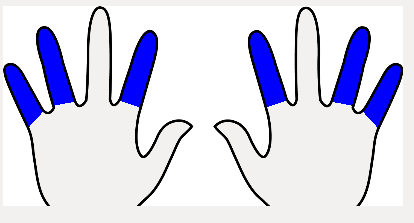
\includegraphics[width=\textwidth]{images/with-hands.png}
    \caption{The polygons with the hands image above.}
    \label{polygons-with-hands}
  \end{minipage}
  \hfill
  \begin{minipage}[b]{0.45\textwidth}
    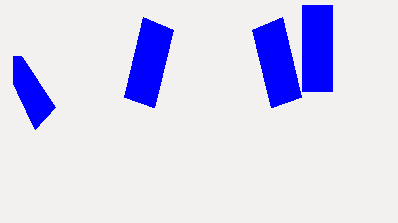
\includegraphics[width=\textwidth]{images/without-hands.png}
    \caption{The polygons without the hands picture above.}
    \label{polygons-without-hands}
  \end{minipage}
\end{figure}


The second part of the interactive keyboard is the keyboard itself.\\
Here is the header file of the tkeyboard class
\begin{lstlisting}
#ifndef TVIRTUALKEYBOARD_H
#define TVIRTUALKEYBOARD_H

//#includes ...

class TVirtualKeyboard : public QWidget {
    Q_OBJECT
public:
    TVirtualKeyboard(TLayouts &layout, QWidget *parent = 0);
    TVirtualKeyboard(const TVirtualKeyboard& orig);

    virtual ~TVirtualKeyboard() {
    }


    QHash<QChar, TVirtualKey*> *getKeys() const {
        return keys_;
    }

    /**
     * Will update the keyboard depending on the
     *  key event (release or pressed)
     * and return the key that was updated
     * 
     * @param ev the key event
     * @return the virtualkey corresponding to the event
     */
    TVirtualKey *updateKeyboard(QKeyEvent *ev, QChar expected = '\0');
    
    
    TVirtualKey *highlightKey(QChar keyChar);


private:
    /**
     * Read the layout's file 
     * and display the keyboard
     * depending on the language
     * 
     * @param lan the language of the keyboard
     * @param country the country code of the keyboard
     */
    void setupWidget(TLayouts &layout);


    /**
     * Will create and add to the layout the
     * TVirtual key from the code of each String
     * and add them to the corresponding line
     * depending on their index in the list :
     * 1 - Number line
     * 2 - Upper line
     * 3 - Baseline
     * 4 - Bottom line
     * 
     * @param keyChars the list of list of key code
     */
    void createKeys(QList<QStringList> keyChars);


    /* All the 'normal' keys that can change of position on the 
     * keyboard
     *  */
    QHash<QChar, TVirtualKey*> *keys_;
    
    /*
     All the 'special' keys that will always be on the same position
     * on the keyboard (spacebar, shift, enter, ...)
     */
    QHash<int,TVirtualKey*> *modifiers_;
};

#endif /* TVIRTUALKEYBOARD_H */
\end{lstlisting}
The virtual keyboard contains a hash where the key is a char and the value is the key to highlight.\\
The key is a simple object that represent a key in the keyboard, it can contains on or several characters to display. For example, all the letters key are containing only one character on the keyboard, whereas the number keys contain at least two chars :
\begin{itemize}
	\item One for the number.
	\item A special character
	\item (Not on all keyboards) Another special character
\end{itemize}

Here is the three differents possibilities of key display :
\begin{figure}[H]
  \centering
  \begin{minipage}[b]{0.10\textwidth}
    
\includegraphics[width=\textwidth]{images/key-one-char.png}
    \label{key-one-char}
  \end{minipage}
  \begin{minipage}[b]{0.10\textwidth}
    
\includegraphics[width=\textwidth]{images/key-two-chars.png}
    \label{key-two-chars}
  \end{minipage}
    \begin{minipage}[b]{0.10\textwidth}
    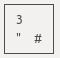
\includegraphics[width=\textwidth]{images/key-three-chars.png}
    \label{key-three-chars}
  \end{minipage}
  \caption{The three different types of key}
\end{figure}

Every time the user type a key on his keyboard, the char typed is retrieved in the hash and highlighted.\\
Depending on the exercise, the key can change its color. The actual possible colors are blue,cyan and red. Here is an example of two colors used on the keyboard : 
\begin{figure}[H]
	\centering
	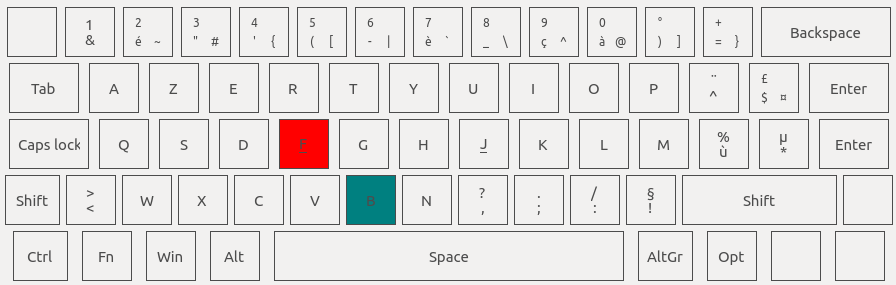
\includegraphics[width=0.7\textwidth]{images/wrong-key.png}
	\label{wrong-key}
	\caption{Different colors on the same keyboard}
\end{figure}

Then to link the keyboard and the hands, the class Tpresentation comes in. It contains a single virtual keyboard and the hands widget.
It can be used in two ways :
\begin{description}
	 \item[Normally :] as it is in the interactive keyboard game. Where the user just type letters on its keyboard and see it highlighted along with the finger.
	 \item[As an example :] as it is for the learning exercise. A key is already highlighted as well as the finger. And the user has to reproduce the example. Any other letter typed is highlighted in red.
\end{description}

To save all the characters to copy, the TPresentation object contains a String. This string is working as a queue. Every time the user type the correct letter, the first character of the string is removed and the new first character is highlighted on the keyboard. Here is the function that will take care of this.
\begin{lstlisting}
void TPresentation::nextCharToCopy() {
    if (!toPress_.isEmpty()) {
        currentExample_ = toPress_[0];//Take the first char
        TVirtualKey* highlighted = keyboard_->highlightKey(currentExample_);//Highlight it
        if (highlighted) {
            positions_->enableFinger(highlighted->associatedFinger());
            toPress_ = toPress_.remove(0,1);//Remove the first char of the string
        }
    } else {//String empty => nothing to copy
        emit allCopied();
    }
}
\end{lstlisting}

This code walkthrough contains only the most interesting parts of the software but does no contain all the code. It is recommended to peruse the code as well as the comments to fully understand how the whole software works.

\chapter{Memory leaks}
The C++ language has a lot of advantages like the speed and the portability. However, there is one drawback that is embarrassing (particularly in security) which is the memory leak. This problem is only possible on languages where the developer manage himself the memory. Which is not the case in Java for example. A memory leak occurs when the developer create an object in a function and a pointer on this object. The object will be saved on the heap of the program. Then if the developer leaves the function without deleting the pointer, the object on the heap will not be deleted and will occupy space uselessly. \\
Fortunately for the group, Qt is taking care of the majority of these pointers. This is especially true for the GUI. Every pointer created that inherits from QWidget, automatically belong to its parent. So, whenever a widget belongs to a dialog or an ephemeral widget, it will be deleted when its parent will be closed. This simplify a lot the programmers life. However, all the classes does not inherit from QWidget. Some pointer deletion had to be made by the group. All the data classes had to be deleted manually when unused.\\
Because sometimes the memory leaks are hard to detect, the group used a very helpful tool compatible with QtCreator called Valgrind. This program could detect various types of memory leaks and problems such as the double deletion.


\chapter{Git and Github integration}
To be able to develop effectively, the group used git for the version control and github.com as a remote server to host the code.\\
The group could choose to create a private repository or a public repository on github. Since the group accepted the Qt's license which state that the code must be open source, they created a public repository.\\
The group member knew the basics of git and were able to develop together without too many problems.\\

\begin{figure}[H]
	\centering
	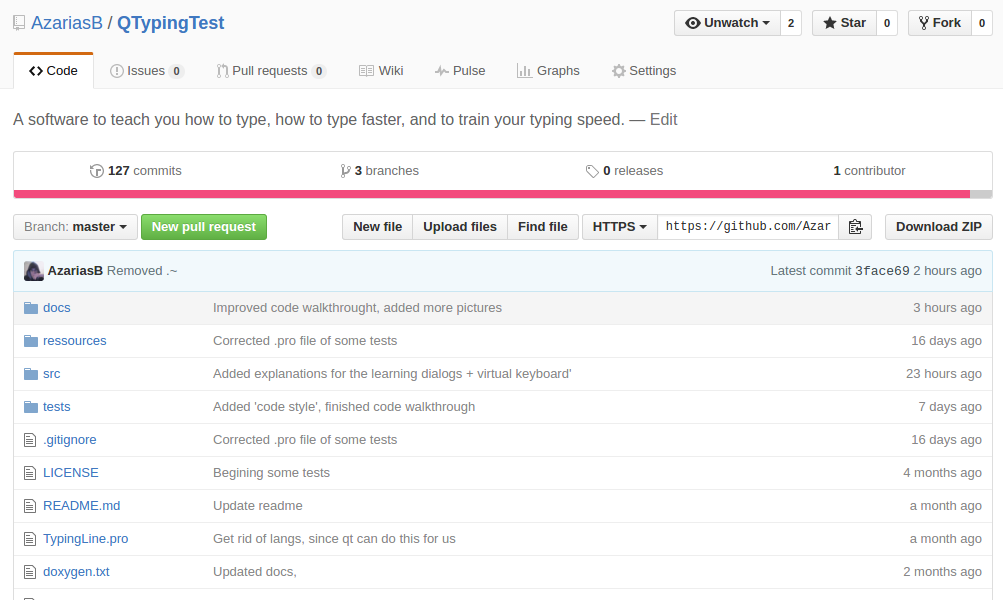
\includegraphics[width=0.7\textwidth]{images/github-main.png}
	\label{github-main}
	\caption{The github page of the project.}
\end{figure}


However, to reduce the number of conflicts on git, the group created three branches :
\begin{description}
	\item[Master  :] the main branch. The software started to get bigger and could contain bug. The aim of this branch was to have only clean code and have a valid base.
	\item[Dev : ] the branch used to develop the software. This was giving the project the possibility to correct bugs before merging with the branch master. This branch was one of the most used of the project. When the part of the software developed on this branch was finished, the group was running all the tests to see if everything was still working and if there were, then this branch was merged with the master branch.
	\item[Stats : ] used only by Pierre while working on the statistics. The purpose of this branch was to work on the statistic page without changing anything else. Unfortunately the result was not successful enough to be integrated to the software and this branche was never merged with the master branch.
\end{description}

Here is the three branches as shown in github :
\begin{figure}[H]
	\centering
	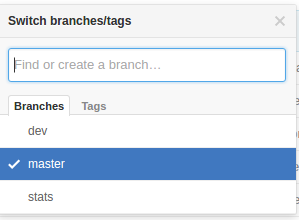
\includegraphics[width=0.7\textwidth]{images/github-branches.png}
	\label{github-branches}
	\caption{The branches on github.}
\end{figure}

The website github as many advantages such as showing the number of line changed in the project over the time. Here is the chart showing how QTypingTest progressed :
\begin{figure}[H]
	\centering
	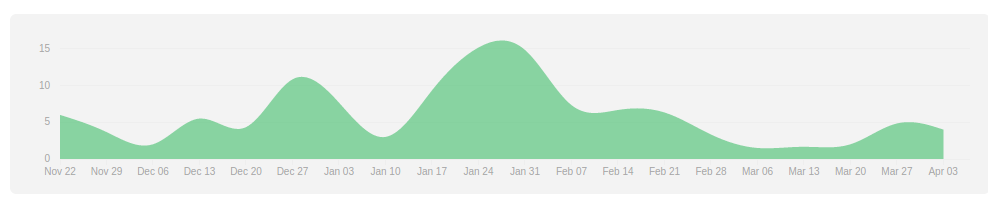
\includegraphics[width=0.7\textwidth]{images/github-progression.png}
	\label{github-chart}
	\caption{The number of line changed (added/deleted) over the time.}
\end{figure}

These two tools : git and github were really useful and accelerated the speed of development of the group.

\chapter{Data design}
All the data is stored in objects when the software is running. Which also mean it is stored in the RAM of the computer.
The problem, is that when the software is not running, the objects are cleared, and not kept in the RAM. The solution the group used to overcome this problem is to use Qt's saving system called QSettings.\\
This figure shows all the user's data to be saved :

\begin{figure}[H]
	\centering
	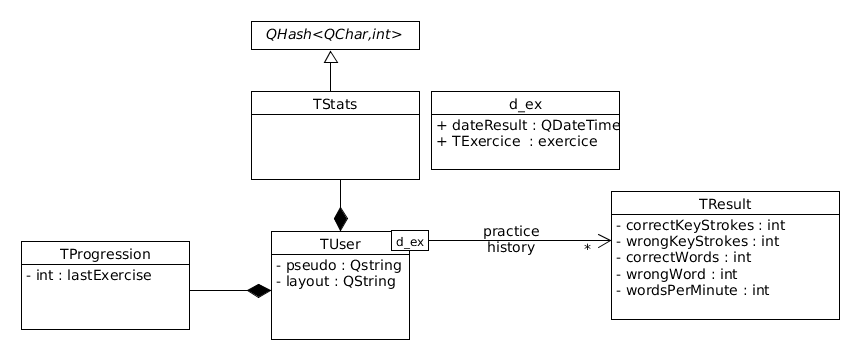
\includegraphics[width=0.7\textwidth]{images/diagram-data.png}
	 \caption{The user's data}
	 \label{diagram-data}
\end{figure}

All the objects represented contains two functions :
\begin{itemize}
	\item One to save the object itself (operator <<)
	\item One to create the object from a save (operator >>)
\end{itemize}

So every time a user was saved, the first function of every object was called, and at the start of the software, all the objects were loaded from the persistent memory to the RAM by calling the second function.\\
Since the model is not complex and a very few object are in relationship, the group chose to use QSettings. \\
However, Qt also supports the database operations and provide a support for sqlLite. As said above, there is also a support for XML and JSON. Those last two were not chosen two prevent easy cheating.


\part{System implementation}
\chapter{Building the software}
\section{First prototype}
The first prototype that the group presented to the first demo was giving an idea of the project. It was really fast to build and was containing only one window, on which the user could write down a text. It was a sort of 'proof of concept'. The purpose of this prototype was to demonstrate the main feature of the software and it was also a starting point for the group.\\
The first prototype was containing only two C++ classes. One for the whole window, and one for each row. Even if the prototype was working well, the interface was not very user-friendly and an offset could easily appear when the user was making too many mistakes.
Meaning that even if the prototype was working, a lot of work would be necessary to improve the user interface. \\
This prototype was also a sort of training for the group, it was the first window ever made with Qt. Because the group members did not know anything about this framework, it was understandable to have such a poor interface.

\section{Second prototype}
The second and actual prototype is a lot more evolved than the first prototype. There are more features, it is working better and is more user-friendly. Of course, there is some improvements that remains possible.\\
However, the software is ready for production and can be used by anyone who wants to.\\
The second prototype started with a big improvement of the first prototype. The two lines : one for the text, and one for the text-field where the user can type, were merged into a single one. So, as the user types the text, the current character is displayed in a certain color, the future characters are also displayed as done. Therefore, the offset problem was solved. Thanks to the support of HTML in the label with Qt, the task was quite easy.\\
Now that the group had a functional and user-friendly base, they could start to work on the other parts of the project and use this base for differents features.\\
Here are the list of features that were developed on this base, by order of development :
\begin{enumerate}
	\item random-letters typing. Were the user has to type a random set of letters
	\item random-words typing. Were the user has to type real words
	\item text typing. Were the user has to type an existing text (written by great authors such as George Orwell)
	\item improvement. This exercise is using the user's statistics to know what mistake is the more frequent
\end{enumerate}
All these different exercises has their own class. They also all inherit from the same base class to have access to the same resources such as a timer, a play/pause button, and a score a the end.\\
Then the group worked on different aspects of the software, such as an interactive keyboard, the user's statistics and a homepage where a user can create and delete his account, connect and disconnect.


\chapter{Current state of the software}
The current state of the software is complete. The software is available on \url{github.com/AzariasB/QTypingTest} and can be downloaded for Linux or Windows. Anyone with a computer can download the software and start to learn how to type !\\
Even if the system is working well, the GUI is improvable. However, since the group is not design students, they did as they could to create a usable software that does not hurt eyes. Furthermore, because the software is made up in C++, it is a bit harder than the web to stylize the interface. Even though Qt provides a CSS-like feature to change the style of every elements in a window.


\part{Testing}
\chapter{Unit testing}
Really early in software development, it became obvious that some key features required unit testing.\\
Luckily Qt provides a way to easily and quickly create unit testing. All the tests of the projects are on the 'test' folder.\\
The tests for this projects were created for two main purpose :
\begin{enumerate}
	\item ensure that features was working as expected
	\item avoid compiling all the project to test a single feature
\end{enumerate}
Some test requires the GUI some does not. The hardest part of the test was not to create them but was to make the software testable. For example, a lots of features held on randomness, and it is not possible (or silly) to test randomness. This means, the less randomness, the more testable. Or pseudo-random features were testable.\\
Here is an example of a test file :

\begin{lstlisting}
//includes [...]
class TestUtils : public QObject {
    Q_OBJECT
private slots:
    void testSurroundAll();
    void testSurroundAt();
    void testRemoveTags();
    void testAbsolutePosition();
};
\end{lstlisting}
First, the test class must be declared. The whole test can be written in a single .cpp file.\\
To be able to run the test on the class, it must inherit from QObject. Then the Qt test framework will run all the
private slots.\\
In this case, the HTML helper is tested. Four functions are created to test it.\\
Here is one of them.

\begin{lstlisting}
void TestUtils::testAbsolutePosition() {
    QString joel_0 = "joel";
    QString joel_1 = "<p>j</p>oel";
    QString joel_2 = "jo<p>e</p>l";
    QString joel_3 = "joe<p>l</p>";
    QString joel_4 = "<p>j</p>o<b>e</b><u>l</u>";
    QString joel_5 = "<b><u>j</b></u>oel";

    qDebug() << "Get the absolute position of a char in a String";
    QCOMPARE(html::getAbsoluteCharPosition(joel_0, 0), 0);
    QCOMPARE(html::getAbsoluteCharPosition(joel_1, 0), 3);
    QCOMPARE(html::getAbsoluteCharPosition(joel_2, 2), 5);
    QCOMPARE(html::getAbsoluteCharPosition(joel_3, 3), 6);
    QCOMPARE(html::getAbsoluteCharPosition(joel_4, 3), 20);
    QCOMPARE(html::getAbsoluteCharPosition(joel_5, 1), 15);
}

//Other functions...

QTEST_MAIN(TestUtils)
#include "testutils.moc"
\end{lstlisting}
Here is how a test function looks like. As a lot of other test framework, there is the initialization part, the action part and the test part. Qt provides functions such as \texttt{QCOMPARE},\texttt{QVERIFY} and others to run the test. To run the test, the file must be compiled and run. In this case, there is no graphics, all is displayed in the console. Here is the output when the entire file is run.

\begin{lstlisting}
********* Start testing of TestUtils *********
Config: Using QtTest library 5.2.1, Qt 5.2.1
PASS   : TestUtils::initTestCase()
QDEBUG : TestUtils::testHTML() Testing HTML 
QDEBUG : TestUtils::testHTML() Adding a single tag 
QDEBUG : TestUtils::testHTML() Adding multiples tags 
QDEBUG : TestUtils::testHTML() Adding attributes 
QDEBUG : TestUtils::testHTML() Remove all the tags 
QDEBUG : TestUtils::testHTML() Remove only the asked tags 
QDEBUG : TestUtils::testHTML() Remove all the tags (no second arguments) 
QDEBUG : TestUtils::testHTML() Get the absolute position of a char in a String 
PASS   : TestUtils::testHTML()
QDEBUG : TestUtils::testFactory() Changing locale for test purpose 
QDEBUG : TestUtils::testFactory() Testing factory (non-random functions) 
QDEBUG : TestUtils::testFactory() ("of", "do", "off", "food") 
QDEBUG : TestUtils::testFactory() ("be") 
QDEBUG : TestUtils::testFactory() ("be", "we", "went", "been", "between", "new", "ten") 
QDEBUG : TestUtils::testFactory() Testing practice generation 
QWARN  : TestUtils::testFactory() Warning : no letters available to generate the practice 
QDEBUG : TestUtils::testFactory() Must contain only real words 
QDEBUG : TestUtils::testFactory() Must contain existing and random words 
QDEBUG : TestUtils::testFactory() Testing that the generation is completely random 
QDEBUG : TestUtils::testFactory() Testing the text generation 
QDEBUG : TestUtils::testFactory() ("into", "a") 
QDEBUG : TestUtils::testFactory() ("into", "one;", "and", "that,", "whilst", "this", "planet", "has", "gone", "cycling", "on", "according", "to", "the", "fixed", "law", "of", "gravity,", "from", "so") 
PASS   : TestUtils::testFactory()
PASS   : TestUtils::cleanupTestCase()
Totals: 4 passed, 0 failed, 0 skipped
********* Finished testing of TestUtils *********
\end{lstlisting}
The series of test is passing, to help the developer identify what part of the test is running, it is possible to output messages.
At the end of the tests, the number of passed, failed an skipped is indicated.

\chapter{GUI testing}
The GUI testing was created to avoid reproducing a big number of steps before being able to carry out the real test. It allows the developer to :
\begin{enumerate}
	\item Test only the part wanted of the software
	\item Avoid wasting time compiling the whole software when only a single part of it tested.
\end{enumerate}

A GUI testing file is consisting of a really few lines, where the window/widget is created, modified and shown. Then all the developer has to do is to directly use the interface to test what he wants.\\
The group did set-up a lots of these test. Every single dialog has its own test file.

%show some code ?

\part{Usability - Users tasks}
\chapter{What can the user do}
The finished software allows the user to do the following tasks:
\begin{itemize}
	\item Start the executable of the software.
	\item Connect to its profile on the homepage.
	\item Create a new user on the homepage.
	\item Delete his profile on the homepage.
	\item Change his settings (alias,keyboard layout, software language)
	\item Select a part of the software were to navigate to
	\item Start a new training on the training page and learn new letters to type.
	\item Unlock the next training exercise if the user was fast enough at the previous one
	\item Start a new practice exercise. The exercise can be one of the following 
	\begin{itemize}
		\item Race : type the most words before the time runs out
		\item Classical : type the given words until the end as fast as possible
		\item Text : type the given text until the end as fast as possible
		\item Improve : type the given words specially chosen from the mistake made during a training
	\end{itemize}
	\item See his statistics at the end of a run :
	\begin{itemize}
		\item Number of words per minute
		\item Number of correct keystrokes
		\item Number of wrong keystrokes
	\end{itemize}
	\item Start the interactive keyboard and see what finger is used to type a certain letter
	\item Disconnect and close the window without losing all his data
\end{itemize}


\chapter{Overall aesthetic}
The software is neither beautiful nor ugly to look. Because this was the first time the group ever used Qt, the main goal was not to create a fully user-friendly interface but a usable, interactive and intuitive interface. Moreover, since the interface look-and-fell changes for each OS, it would have been hard to create a unified interface for all the OS. Biggest effort in therm of aesthetic were made for the look-and-feel of the exercise/training window thus the user can instantly understand how the cursor is moving and when the given answer is correct or wrong. This particular interface will not change, no matter what is the OS, because it has been wittingly chosen to appears like this:
\begin{itemize}
	\item The color of the font
	\item The size of the font
	\item The font itself (monospace)
\end{itemize}
All others part of the software will depend on the OS. For example the font of the button will be \textit{Ubuntu} for the Ubuntu OS, but it will be \textit{Verdana} for windows. Same thing for the button. They will look flatter on windows 10 than on Ubuntu.


\part{Conclusion and further work}
\chapter{Project result}
In order to determine how successful the project was, it is important to look back at the goals which were set at the beginning of it. These goals are outlined in the project proposal.\\
Here is the list of what these goals were :

\begin{itemize}
	\item Learn how to use Qt framework.
	\item Create a free software with Qt.
	\item Let the source code open and free for all on Github.
	\item Create a software that can teach you how to improve your typing skills.
	\item Allow different keyboard layouts.
	\item Translate this software in different languages.
\end{itemize}

All these requirements has been met except the last one which was to translate the software into different languages.\\
The group succeeded to create an adaptable software who will automatically change its configuration depending on the user's computer. Event if, for now, only two languages are available, anyone can create a file with the most common words of his language and insert it into the software without having to change anything in the code. The same goes for the texts and the keyboard layouts. Only two languages are available but anyone can easily type new texts or create a new JSON file for the layout and insert them into the software without having to change anything in the code.\\
Because the software is made for private use and does not contain any sensible informations, there is no security, only a simple login system without password.\\
The software is compiled in release mode en ready for distribution on Windows OS, Ubuntu and Mac OS.

\chapter{Possible improvements}
Here is a list of the possible improvements for the software :
\begin{itemize}
	\item Correct all memory leaks. Even if the group made all its possible to correct the most of them, some remains and may slow down the software.
	\item Improve the user interface. Minimum was made to make the interface usable but a lot of improvement are possible.
	\item Create more games to get funny way to learn. The software is a bit to formal and not really appropriate for kids.
	\item Allow the user to race with other people (on the same computer or online) because playing all alone can be boring. When comparing the speed with someone else, this could motivate the user to train more and more to win at these races.
	\item Add statistics. For now, a user has an history of exercises made, but these are not displayed. This means the user can only see result of the exercise at the end of it and then does not have any way to know improvements made.
	\item Create more practice mode. A strong and usable base was made for practice exercise, and a lot more game modes could be created with a very few lines of code. For examples, a mode where at each wrong keystrokes typed, the final time would be increased. This would push the user to focus on the accuracy rather than the speed.
\end{itemize}


\chapter{Further work}
If the group were to continue developing this software, then there are a few things to aim for.\\
First of all, use Qt a better way. Even if a lot of features of Qt were used, the group may have missed a lots of them. A simple example is user's interface design where only the basic features were used. Qt is really powerful and during this project, the group only had the opportunity to brush the possibilities of Qt. This framework is almost a other language because of its magnitude.\\
A better C++ code would be another aim of the group. The actual code is not perfect and could be improved to be more flexible and more maintainable. Furthermore, improving the C++ quality code would reduce the number of memory leaks of the software and so improve the speed of the software.\\
The documentation of the project is generated thanks to a program called Doxygen. Only the basics options are enabled on this program. Doxygen allows options that the group did not use and could make the documentation more readable.\\
Lastly, a little website to distribute the software would be a great plus to the software. Since it is only available on github which is mainly for developers, the individuals won't be able to download it easily. The website would give an easy access to anyone who wants to use the software without having to go through Github.\\